\documentclass[10pt,landscape,a4paper]{article}
\usepackage{multicol}

\usepackage[sfdefault]{roboto}
\usepackage[T1]{fontenc}


\usepackage[landscape]{geometry}
%\usepackage{hyperref}
\usepackage[utf8]{inputenc}
\usepackage{minted}
\setminted{fontsize=\tiny}
\setmintedinline{fontsize=\tiny}
\usepackage{graphicx}
%\usepackage[binary-units]{siunitx}
%\usepackage[usenames]{xcolor}

\newcommand{\css}[1]{\mintinline{css}{#1}}
\newcommand{\html}[1]{\mintinline{html}{#1}}
\newcommand{\js}[1]{\mintinline{js}{#1}}

\geometry{top=1cm,left=1.5cm,right=1cm,bottom=1cm}

% Turn off header and footer
\pagestyle{empty}
 
% Redefine section commands to use less space
\makeatletter
\renewcommand{\section}{\@startsection{section}{1}{0mm}%
                                {-1ex plus -.5ex minus -.2ex}%
                                {0.5ex plus .2ex}%x
                                {\normalfont\large\bfseries}}
\renewcommand{\subsection}{\@startsection{subsection}{2}{0mm}%
                                {-1explus -.5ex minus -.2ex}%
                                {0.5ex plus .2ex}%
                                {\normalfont\small\bfseries}}
\renewcommand{\subsubsection}{\@startsection{subsubsection}{3}{0mm}%
                                {-1ex plus -.5ex minus -.2ex}%
                                {1ex plus .2ex}%
                                {\normalfont\footnotesize\bfseries}}
\renewcommand{\paragraph}{\@startsection{paragraph}{3}{\z@}%
                                {-1ex plus -.5ex minus -.2ex}%
                                {-.5em}%
                                {\normalfont\scriptsize\bfseries}}
\makeatother

% Don't print section numbers
\setcounter{secnumdepth}{0}

\setlength{\parindent}{0pt}
\setlength{\parskip}{0pt plus 0.5ex}

% Compact lists
\usepackage{enumitem}
\setlist{nosep}

% -----------------------------------------------------------------------

\begin{document}

\tiny
\begin{multicols*}{4}

% multicol parameters
% These lengths are set only within the two main columns
%\setlength{\columnseprule}{0.25pt}
\setlength{\premulticols}{1pt}
\setlength{\postmulticols}{1pt}
\setlength{\multicolsep}{1pt}
\setlength{\columnsep}{2pt}

\section{CSS}

\subsection{Diverses}

\begin{description}
\item[box model] content, padding, border, margin. \\
  \css{box-sizing: border-box;} damit padding / border zu
  width/height zählen.
\item[vererbt] color, font-*, text-indent, text-align, cursor, list-style
\item[vw, vh] 1 vw/vh = 1\% viewport width/height
\item[rem/em] Relativ zu root/html (rem) oder parents. Default: 16px = 1rem = 1em
\item[float] Mit \css{float: left|right} fliesst Text darum; nach \css{clear:
    both|left|right;} wieder darunter.
\item[position] \css{fixed}: Always visible, relative to viewport.
  \css{absolute}: No space, relative to ancestor/containing block.
  \css{relative}: No space, relative to itself.
\end{description}

\subsection{Display}
  \begin{description}
    \item[inline] margin/padding nur links/rechts, ignoriert width/height,
      andere Elems auf selber Zeile.
    \item[block] Element füllt ganze Zeile
    \item[inline-block] Inline aber mit block-Features (width/height/etc.)
    \item[none] Wird entfernt, kriegt keinen Platz (\css{visibility: hidden}:
      Platz bleibt)
  \end{description}
\subsection{Selektoren}

\begin{description}
\item[Attribut] \css{input[type=submit]}
  \begin{description}
  \item[start] \css{[a|=v]} (words), \css{[a^=v]}
  \item[end] \css{[a$=v]} %$
  \item[contains] \css{[a~=v]} (words), \css{[a*=v]}
  \end{description}
\item[ID] \mintinline{css}{#my-id}
\item[Klasse] \css{.my-class}
\item[Nachfahren (irgenwann) / Kind (direkt)] \css{p a}, \css{p > a}
\item[Geschwister / Nachbarn] \css{p ~ a}, \css{p + a}
\item[Pseudo-Elemente] \strut \\ \css{::before}, \css{::after}, \css{::first-line},
  \css{::first-letter}, \css{::selection}
\item[Pseudo-Klassen] \css{:first-child}, \css{:last-child},
  \css{:nth-[last-]child(2nd|odd|even)}, \css{:empty}, \css{:hover}, \css{:active},
  \css{:focus}, \css{:visited}, \css{:not()}, \css{:contains('text')} (jQuery)
\end{description}

\subsection{Titel-Nummerierung}

\begin{minted}{css}
body { counter-reset: ctr; }
h3:before { counter-increment: ctr; content: counter(ctr); }
\end{minted}

\subsection{Spezifität (a b c)}

\begin{description}
  \item[a] ID selectors (\mintinline{css}{#ex})
  \item[b] Class selectors (\css{.ex}), attribute selectors (\css{[type="ex"]}), pseudo-classes (\css{:hover}))
  \item[c] Tag/type selectors, pseudo-elements
\end{description}

Universal-Selektor \css{*} wird ignoriert, bei \css{:not(...)} werden nur die Inhalte gezählt.

\css{!important} und inline-Styles gewinnen immer.


\section{UCD}
Untere beide Garrett-Ebenen, \textbf{Umfang (Inhaltsanforderung)} mit Anforderungsanalyse.
\textbf{Strategie (Nutzerbedürfnisse)} mit Marktanalyse, Zielgruppenanalyse

Benutzerbefragung ist kein User Centered-Design, Nutzer wissen eigentlich
nicht was sie wollen.

Wichtige Axiome: Benutzer sind Experten in ihrem Kontext und in ihrer
Welt. Designer und Techniker sind Experten darin, wie die Welt sein
könnte. Vor dem besser machen, muss die alte Welt verstanden werden.

\begin{description}
  \item[Analyse] Benutzer und Kontext verstehen
  \item[Modellieren] Entwurf und Optimierung einer passenden Lösung
  \item[Spezifikation] die Lösung in die Entwicklung tragen
  \item[Realisierung] (Unterstützung bei der) Implementierung der Lösung
  \item[Evaluation] Resultate mit Benutzern überprüfen
\end{description}

\section{MVC example}

\begin{minted}{js}
function createToDosDataService() {
  return {getToDos: function (cb) { $.get('/api/toDo', cb); },
          createNewToDo: ... }}}
function createToDosViewController(toDosDataService, jQRenderTarget) {
  const createToDosViewHTML = Handlebars.compile($('#index-view').html());
  
  function createToDosViewController(toDosDataService, jQRenderTarget) {
    const toDosViewController = {
      initView: function () {
        toDosDataService.getToDos(
            toDosViewController.renderToDosToTarget);
        jQRenderTarget.on('click', '[data-click=1D]', (e) => {...}
      ...}

$(function () {
    const toDosDataService = createToDosDataService();  // s
    const jQRenderTarget = $('#appContainer');  // t
    const toDosViewController = createToDosViewController(s, t);
    toDosViewController.initView(); });
\end{minted}

\vfill \columnbreak

\section{HTML}

\subsection{Skeleton}

\begin{minted}{html}
<!DOCTYPE html>
<html lang="de">
  <head>
    <meta charset="utf-8">
    <meta name="author/publisher/description" content="Ich">
    <title>foo</title>
    <link rel="icon" href="favicon.png" type="image/png">
    <link rel="stylesheet" type="text/css" href="style.css">
    <script src="foo.js"></script>
  </head>
  <body>
    <header><h1>[Seitentitel]</h1></header>
    <nav>[Navigation]</nav>
    <main><article>[Artikel] <small>[Autor]</small></article></main>
    <aside>[Werbebanner]</aside>
    <footer>
      <address>[Kontakt]</address>
      <time datetime="16-07-08">[Änderung]</time>
    </footer>
  </body>
</html>
\end{minted}

\subsection{Figures / Images}
\begin{minted}{html}
<figure>
  <!-- width: of source -->
  <img src="foo.jpg" alt="blabla" width="123">
  <figcaption>Text unter der Figure</figcaption>
</figure>
<picture>
  <source type="image/jpeg" srcset=""> <!-- more sources -->
  <img src="..."> <!-- fallback -->
</picture>
\end{minted}

\subsection{Tables}

\begin{minted}{html}
<table>
  <caption>Conference Schedule</caption>
  <thead>
    <tr>
      <th scope="col">Time</th>
      <th scope="col">Track 1</th>
      <th scope="col">Track 2</th>
    </tr>
  </thead>
  <tbody>
    <tr>
      <th scope="row">08:30 - 10:00</th>
      <td colspan="2">Coffee</td>
    </tr>
    <!-- ... -->
  </tbody>
</table>
\end{minted}

\subsection{Forms}

\begin{minted}{html}
<form action="sendmessage.php" method="post">
  <label>Male
    <input type="radio" name="gender" value="male" checked>
    <!-- ... -->
  </label>
  <label for="phone">Phone</label>
  <input type="tel" name="phone-number" id="phone" required> 
  <input type="text" name="cust-nr" placeholder="CH12" pattern="<regex>">
  <select name="message-type">
    <option value="feedback" selected>Feedback</option>
    <option value="question">Question</option>
  </select>
  <fieldset>
    <legend>Options</legend>
    <!-- ... -->
  </fieldset>
  <button type="submit">Submit</button>
  <button type="reset">Reset</button>
</form>
\end{minted}

\subsection{Misc}

\begin{minted}{html}
<video controls poster="thumb.png">
    <source src="media/TI-Nspire_CX_CAS_3D_Model.mp4" type="video/mp4">
    <track kind="subtitles" src="sub.en.vtt" srclang="en" label="English">
    Fallback message/link/...
</video>  <!-- object: neuer, browser entscheided selbst -->
<object data="foo.svg" type="image/svg+xml" role="img"></object>
<iframe src="https://www.youtube.com/embed/..." allowfullscreen></iframe>
<dl><dt>Term</dt><dd>Desc</dd><dd>Desc2</dd></dl>
\end{minted}


\section{JavaScript}

\begin{minted}{js}
false, 0, "", null, undefined, NaN  // falsey
'0', 'false', {}, []  // truey
isNan(0 / 0) -> true  // NaN
3/0 -> Infinity (-Infinity)  // Infinity
.length, .slice(), .trim(), .indexOf(), .match(/re/), .replace()  // str
function foo(arg, ...args)     arguments, [...arguments] // as array
for (let x in obj):  // foreach - property names
for (let x of arr):  // foreach - values
typeof(myvar) === 'undefined'  // undefined
.length, .forEach(fn), .map()/.filter()  // arrays
const arr = [1,2,3,4].map(x => x*x)  // lambda
(function() { ... }());  // IIFE
console.log(`v=${v}`)  // ES6 string formatting
{"a": a, "b": b} == {a, b}  // ES6 object short form
const { left, top } = foo();  // ES6 destructuring assignment
/JS/i.text('foo')  // Regex; or via string API
promiseFactory().then(callback).catch(errorcb)  // promises
"3" + 2 == 3 + "2" == "32"  // wtf
\end{minted}

\begin{description}
  \item[scope] function mit \js{var}, block mit \js{const}/\js{let}
  \item[Hoisting] Dekl. (nicht Init!) an Scope-Anfang. ``Temporal
    dead zone'' mit \js{let}/\js{const}.
  \item[Semicolon ins.] Wenn concat. Zeile fehlerhaft
\end{description}

\vfill

\begin{multicols*}{2}
\subsection{Object}
\begin{minted}{js}
function Rect(width, height) {
  this.x = width;  // public
  let y = height;  // private
  this.area = () => this.x * y;
}  // new: Sets {} as 'this'
const rect = new Rect(5, 5);
\end{minted}

\vfill \columnbreak
\subsection{Closure}

\begin{minted}{js}
function counter(start) {
  return function() {
    start = start + 1;
    return start; }}
const counter0 = counter(10);
console.log(counter0());
\end{minted}
\end{multicols*}

\subsection{Equality}
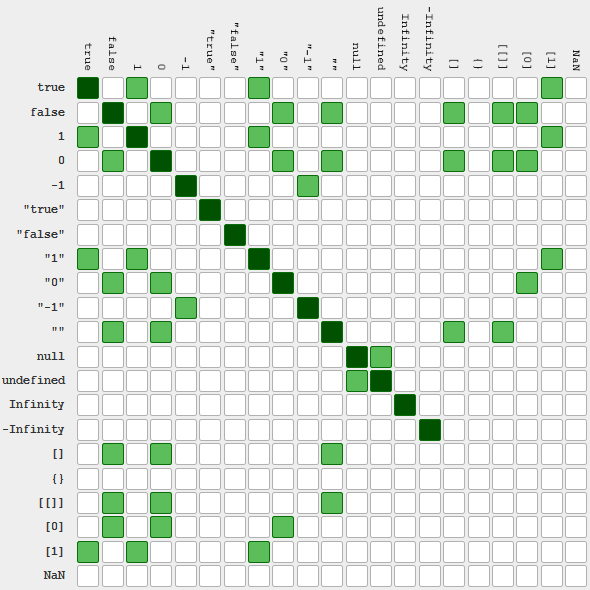
\includegraphics[width=0.8\columnwidth]{jstruth.png}

\subsection{DOM API}

\begin{minted}{js}
document.createElement(tagName) -> Node
document.createTextNode(text) -> Node
document.createAttribute(attributeName) -> Node
document.getElementsByTagName/ByClassName(name) -> NodeList // live
document.getElementById(id) -> NodeList
document.querySelector[All](selector) -> Node[List]

node.childNodes[x] // contains text nodes!
node.firstElementChild/lastElementChild/nextElementSibling
node.nodeName/nodeType/nodeValue
node.appendChild(node)

elem.id/tagName/attributes/className/innerHTML/outerHTML/textContent
elem.insertAdjacentHTML/Text/Element(pos, elem)
// pos: 'beforebegin', 'afterbegin', 'beforeend', 'afterend'
elem.removeChild(node)
elem.appendChildNode(node)
elem.insertAfter(childNode, newNode)

window.onload = function() { /* DOM manipulation here */ };
window.onload = null;
button.addEventListener('click', handler)
button.removeEventListener('click', handler)
ev.stopPropagation() // stop bubbling
ev.target  // original target element
// 'this' in element: element on which the listener was registered
\end{minted}

\columnbreak

\subsection{jQuery}

\begin{minted}{js}
$('p').parent().prop('tagName');  $('p > span').nth(2).next();
// Elements (val/text/html: get or set!):
.val() /* forms */, .text(), .html(), .append(), .replaceWith()
$('<ul><li>foo</li></ul>')  // New element
// Set CSS / properties:
$('#foo').css('font-style', 'italic')  $('#foo').prop('disabled', true)
// Events ('change', '[dbl]click', 'mouse[down|up|enter|leave|move]):
// 'focus', 'blur', 'keydown', 'keyup', 'keypress')
$('body').on('click', 'button' /* opt. filter */, handler)
$('body').off(handler); $('body').once(handler);
jQuery.noConflict(); (function($) { $(...) })(jQuery);
\end{minted}

\subsection{XHR / Ajax}

\begin{minted}{js}
let req = new XMLHttpRequest();
req.onreadystatechange = function() {
  if (req.readyState == 4 && req.status == 200 /* also status 201/304? */) {
    handleResult(req.responseText, req.responseXML); } }
req.open('GET', 'http://example.com', true /* async */);
req.send(/* data */);
req2.open('POST', 'http://www.example.com');
req2.setRequestHeader('Content-Type', 'application/x-www-form-urlencoded');
\end{minted}

\subsubsection{Ajax with jQuery}

\begin{minted}{js}
$.ajax({type: 'POST', dataType: 'html', url: 'some/url/',
        data: { ...}).done(function(data, jqXHR) { ... });
$.get('some/url/', function(data, [textStatus, jqXHR]) { ... });
$.post('some/url/', postData, function(data, ...) { ... });
// Promise methods
.done(function(data, jqXHR) { ... })
.fail(function(jqXHR, textStatus, error) { ... });
.always(function(data|jqXHR, status, jqXHR|error) { ... });
\end{minted}

\subsection{Handlebars}

\begin{minted}{handlebars}
<script id="customersTemplate" type="text/x-handlebars-template">
  {{#each this}}
    <li> {{ firstName }} {{ lastName }} </li>  <!-- this.firstName -->
  {{/each}} {{dateFormat this.dueDate 'MM DD'}}  <!-- calling helper -->
</script>
\end{minted}
\begin{minted}{js}
const customers = [{firstName: 'Peter', lastName: 'Pan'}]

const customersTemplate = $("#customersTemplate").html();
const createCustomersHtml = Handlebars.compile(customersTemplate);

$(document.body).append(createCustomerHtml(customers));
\end{minted}

\section{Usability}

\subsection{Stone}
\begin{description}
\item[Visibility]  Der erste Schritt zum Ziel ist sichtbar.
\item[Affordance] Begreifbarkeit, Resultat ist vorhers.
  \item[Feedback] Es ist klar was passiert (ist)
  \item[Simplicity] Nicht mehr als nötig für die Aufgabe
  \item[Structure] Logische/konsistente Organisation
  \item[Consistency] Vorhersagbarkeit durch Konsistenz
  \item[Tolerance] Fehler vermeiden, easy recovery
  \item[Accessibility] Design für alle Personengruppen \& Situationen
\end{description}

\subsection{Garrett}
\begin{description}
  \item[Oberfläche] Attraktiv, Vertrauenserweckend $\rightarrow$ Farben, Schriften, Icons
  \item[Raster] Erwartungskonform, fehlertolerant, effizient $\rightarrow$
    Augenführung, Ausrichtung, Interaktionsdesign mit Wireframes
  \item[Struktur] Aufgabengerecht, fe., effi. $\rightarrow$
    Interaktionsdesign (Szenarios), Navigation, Cardsorting
  \item[Umfang] Zielgruppengerecht, effektiv $\rightarrow$ Anforderungsanalyse,
    feature reduction
  \item[Strategie] Marktgerecht $\rightarrow$ Markt-/Zielgruppen-analyse mit Personas
\end{description}

\subsection{Prinzipien der Dialoggest. ISO 9241-110}
\begin{description}
  \item[Aufgabenangemessenheit] Benutzer erledigen Aufgaben effektiv und
    effizient.
  \item[Selbstbeschreibungsfähigkeit] Dialogschritte sind durch Beschreibungen
    oder Rückmeldungen verständlich erklärt.
  \item[Steuerbarkeit] Benutzer kann Richtung und Geschwindigkeit der Interaktion beeinflussen.
  \item[Erwartungskonformität] Dialog entspricht den Kenntnissen des Benutzers.
  \item[Fehlertoleranz] Trotz erkennbarer fehlerhafter Eingaben des Benutzers
    kann das Ziel effizient erreicht werden.
  \item[Individualisierbarkeit] Interaktion kann angepasst werden.
  \item[Lernförderlichkeit] Erlernen der Anwendung wird unterstützt.
\end{description}

  
\end{multicols*}
\end{document}